\chapter{Theoretische Grundlagen} %TODO
Alle benötigten theoretischen Grundlagen relativ kurz gehalten.
Statt Grundlagenwissen zu präsentieren, eher auf die entsprechenden Quellen verweisen.

Jede Untersektion sollte in 1-2 Seiten machbar sein.

\section{Pepper} %TODO
Eine kurze Erklärung zu Pepper und ihren Funktionen/Sensoren.

\section{Choregraphe} %TODO
Eine Überblick zur aktuellen Programmierung von Pepper?
Etwas unsicher, ob das in meine Arbeit passt.

\section{NaoQi} %TODO
Beschreibung der Python-Schnittstelle von Pepper und der 

\section{Blockly} %TODO
\begin{figure} %TODO Löschen, wenn erstes Bild eingefügt
	\centering
	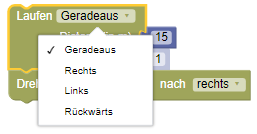
\includegraphics[width=5cm]{Plots/zz-placeholder.png}
	\caption{Platzhalter für Abbildungsverzeichnis.}
	\label{fig:placeholder}
\end{figure}
Eine kurze Erklärung zu den Grundlagen von Blockly.
Kurzer Einblick in die Anwendung von Blockly in Schulen und Lern-Kontexten.\cite{Winterer2020ExpertRABIRP}

\section{Iterative Entwicklung} %TODO
Kurze Einführung in die Theorie der iterativen Softwareentwicklung\cite{Arnowitz2010EffectivePSM}.